\begin{frame}
\frametitle{What is AI?}


\begin{columns}[T]
    \begin{column}[T]{0.44\textwidth}
    \begin{itemize}
    \setlength{\itemsep}{2mm}
        \item AI (artificial intelligence) is a catch-all phrase for any method that appears to mimic a task that requires human intelligence.
        \item It may be divided into specialist \textit{Narrow AI} or \textit{Artificial General Intelligence} (\textit{AGI}, which does not exist yet).
        \item Most current AI uses \textit{machine learning}.
    \end{itemize}
           
    \end{column}


    \begin{column}[T]{0.55\textwidth}
    \vspace{-3mm}
        \begin{center}
            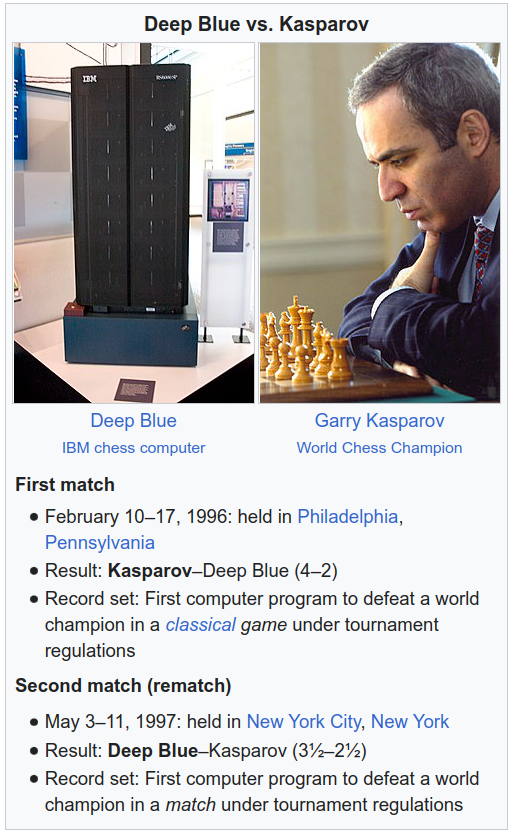
\includegraphics[width=0.75\textwidth]{./misc_images/deep_blue}
        
    \end{center}

    \end{column}
\end{columns}

\end{frame}